\ifSTANDALONE
\section{Wirkungsweise} \label{wirkungsweise}
\fi
\ifEMBED
\subsection{Wirkungsweise} \label{wirkungsweise}
\fi

\ifEMBED
    % Dieses Kapitel ist eine Zusammenarbeit der Gruppen \BLDCTeams. 
    \BLDCcollab
\fi
    
    Schrittmotoren oder auch Stepper genannt, sind Synchronmotoren, bei 
    welchen der Rotor um einen bestimmten Winkel gedreht werden kann. So ist 
    die Rotorposition ohne zusätzliche Sensoren bekannt. Dabei ist zu 
    beachten, dass der Motor keine Schritte verliert, was bei Überlast 
    geschehen kann. Da die meisten Schrittmotorensysteme Open- Loop Systeme 
    sind, entsteht eine dauernde Positionsabweichung bei einem Schrittverlust. 
    Grundsätzlich wird zwischen zwei Schrittmotortypen unterschieden: 
    \begin{itemize}
       	\item Permagnentmagnetmotor
       	\item Reluktanzmotor
    \end{itemize} 
    Der Permanentmagnetmotor besitzt als Rotor einen Permagnentmagneten. Beim 
    Reluktanzmotor besteht der Rotor aus einem gezahnten Weicheisenkern. 
    Permanentmagnetmotoren erreichen eine kleinere Schrittfrequenz, besitzen 
    jedoch ein grösseres Drehmoment als der Reluktanzmotor. Die Kombination 
    aus Reluktanzmotor und Permanentmagnetmotor ist ein Hybridmotor. Ein 
    Hybridmotor verbindet die Vorteile von Reluktanz- und Permagnentmotor.
    
    Der Vollschrittbetrieb kann einphasig oder auch zweiphasig gesteuert 
    werden. Beim einphasigen Vollschrittbetrieb sind immer zwei gegenüber 
    liegende Pole aktiv. Beim zweiphasigen Vollschrittbetrieb werden jeweils 
    zwei nebeneinander liegende Pole aktiv. Im Halbschrittbetrieb werden die 
    beiden Vollschrittbetriebsarten kombiniert. So kann der Schrittwinkel 
    halbiert werden. Zusätzlich kann der Schrittmotor mit Mikroschritten 
    betrieben werden. Dabei folgt der Strom der sinusförmigen 
    Referenzspannung. (Vgl. Seite \pageref{stromgesteuert})
    \begin{figure}[H]
    	\centering
    	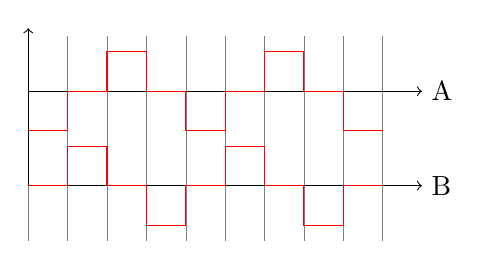
\begin{tikzpicture}
        % Hilfslinien
        \foreach \i in {0, 0.5, ..., 4.5}
        {
            \draw[ultra thin, gray] (\i, 1.9) -- (\i, -0.7);
        }
        % Achsen
    	\draw[->]	(0, 0) -- (0, 2);
    	\draw[->]	(0, 1.2) -- (5, 1.2) node[right]{A};
    	\draw[->]	(0, 0) -- (5, 0) node[right]{B};
        % Kurven
        \draw[red] 
            (0     ,0.7) --
            (0.5   ,0.7) --
            (0.5   ,1.2) --
            (1     ,1.2) --
            (1     ,1.7) --
            (1.5   ,1.7) --
            (1.5   ,1.2) --
            (2     ,1.2) --
            (2     ,0.7) --
            (2.5   ,0.7) --
            (2.5   ,1.2) --
            (3     ,1.2) --
            (3     ,1.7) --
            (3.5   ,1.7) --
            (3.5   ,1.2) --
            (4     ,1.2) --
            (4     ,0.7) --
            (4.5   ,0.7);
        \draw[red] 
            (0      ,0) --
            (0.5    ,0) --
            (0.5    ,0.5) --
            (1      ,0.5) --
            (1      ,0) --
            (1.5    ,0) --
            (1.5    ,-0.5) --
            (2      ,-0.5) --
            (2      ,0) --
            (2.5    ,0) --
            (2.5    ,0.5) --
            (3      ,0.5) --
            (3      ,0) --
            (3.5    ,0) --
            (3.5    ,-0.5) --
            (4      ,-0.5) --
            (4      ,0) --
            (4.5    ,0) ;
    	\end{tikzpicture}
    	\caption{Vollschritt}
    	\label{fig:vollschritt}
    \end{figure}
    
    \begin{figure}[H]
     	\centering
     	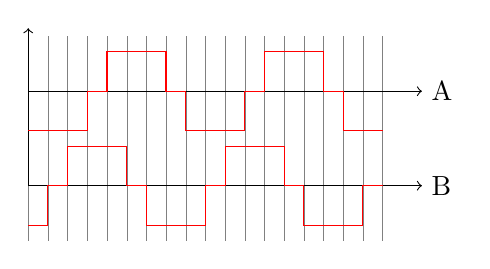
\begin{tikzpicture}
        % Hilfslinien
        \foreach \i in {0, 0.25, ..., 4.5}
        {
            \draw[ultra thin, gray] (\i, 1.9) -- (\i, -0.7);
        }
        % Achsen
    	\draw[->]	(0, 0) -- (0, 2);
    	\draw[->]	(0, 1.2) -- (5, 1.2) node[right]{A};
    	\draw[->]	(0, 0) -- (5, 0) node[right]{B};
        % Kurven
        \draw[red] 
            (0     ,0.7) --
            (0.75   ,0.7) --
            (0.75   ,1.2) --
            (1     ,1.2) --
            (1     ,1.7) --
            (1.75   ,1.7) --
            (1.75   ,1.2) --
            (2     ,1.2) --
            (2     ,0.7) --
            (2.75   ,0.7) --
            (2.75   ,1.2) --
            (3     ,1.2) --
            (3     ,1.7) --
            (3.75   ,1.7) --
            (3.75   ,1.2) --
            (4     ,1.2) --
            (4     ,0.7) --
            (4.5   ,0.7);
        \draw[red] 
            (0      ,-0.5) --
            (0.25   ,-0.5) --
            (0.25   ,0) --
            (0.5    ,0) --
            (0.5    ,0.5) --
            (1.25   ,0.5) --
            (1.25   ,0) --
            (1.5    ,0) --
            (1.5    ,-0.5) --
            (2.25   ,-0.5) --
            (2.25   ,0) --
            (2.5    ,0) --
            (2.5    ,0.5) --
            (3.25   ,0.5) --
            (3.25   ,0) --
            (3.5    ,0) --
            (3.5    ,-0.5) --
            (4.25   ,-0.5) --
            (4.25   ,0) --
            (4.5    ,0) ;
     	\end{tikzpicture}
     	\caption{Halbschritt}
     	\label{fig:halbschritt}
    \end{figure}
    \begin{figure}[H]
    	\centering
    	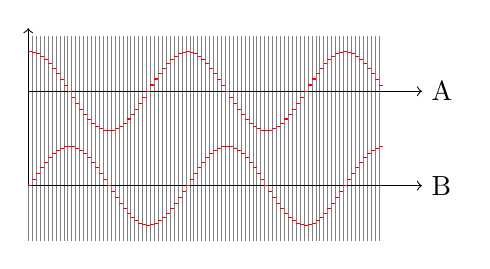
\begin{tikzpicture}
        % Hilfslinien
        \foreach \i in {0, 0.05, ..., 4.5}
        {
            \draw[ultra thin, gray] (\i, 1.9) -- (\i, -0.7);
        }
        % Achsen
    	\draw[->]	(0, 0) -- (0, 2);
    	\draw[->]	(0, 1.2) -- (5, 1.2) node[right]{A};
    	\draw[->]	(0, 0) -- (5, 0) node[right]{B};
        % Kurven
        \foreach \i in {0, 0.05, ..., 4.5}
        {
            \draw[red] (\i, {0.5*sin(180*\i)})          -- (\i+0.05, {0.5*sin(180*\i)});
            \draw[red] (\i, {0.5*sin(180*\i+(90))+1.2}) -- (\i+0.05, {0.5*sin(180*\i+(90))+1.2});
        }
    	\end{tikzpicture}
    	\caption{Mikroschritt}
    	\label{fig:mikroschritt}
    \end{figure}
    Eine Phase sind jeweils die zusammengeschalteten Statorwicklungen. Der 
    unipolare Schrittmotor besteht aus vier Phasen. Ein Elektromagnet besteht 
    aus zwei Phasen, welche gegenseitig gewickelt sind. So kann vermieden 
    werden, dass der Stromfluss durch die Wicklung gedreht werden muss. Der 
    Bipolare Schrittmotor besteht aus nur zwei Phasen. Es muss mit einer 
    Brückenschaltung die Richtung des Stromes gedreht werden. In den meisten 
    Anwendungen werden Bipolare Schrittmotoren verwendet, da ein bipolarer 
    Schrittmotor ein grössseres Drehmoment erzeugt als ein gleich grosser 
    unipolarer Schrittmotor. Die beiden Betriebsarten sind in der 
    \autoref{fig:uniVsbi} ersichtlich. 
    \begin{figure}[H]
       	\centering
       	\includegraphics[width=12cm]{src/Bilder/uniVsbi.JPG}
       	\caption{bipolarer und unipolarer Betrieb}
       	\label{fig:uniVsbi}
    \end{figure}
    
       
    
